\chapter{Heuristics Algorithms}

\section{Introduction}
Meta-heuristics is a sub domain of the artificial intelligence domain. It evolved out of a need for more efficient search techniques with regard to hard problems. 

Meta-heuristics forms part of a collective body of algorithms that use heuristics to search a particular domain's problem space, for the most optimal solution adhering to certain hard and soft constraints. Some of the most important Algorithms that form part of this collective body is:
\begin{itemize}
\item Tabu Search
\item Simulated Annealing
\item Genetic Algorithm
\end{itemize}
The above mentioned algorithms aren't the only algorithms to form part of this sub-domain, but they are the algorithms that have received the most attention in the literature and generally produce good results \cite{SweepMeta}.

In this chapter our main focus will be to discuss each of the above listed algorithms. We will start of by briefly discussing the characteristics of meta-heuristic algorithms after which we will discuss each of the above algorithms in detail. We will also provide a literature study for each algorithm in order for us to see how an algorithm needs to be changed and optimised for a particular problem domain. 

\section{Characteristics of Meta-heuristics}
NP-Complete problems have been proven to not be solvable in polynomial time by traditional search methods such as A* search, Breath First Search and Depth-First Search. Meta-heuristic algorithms on the other hand are much more efficient in searching the problem space and produce much better results in a short amount of time. 

These algorithms are considered to be \emph{general-purpose} algorithms and can thus be applied to a wide variety of optimization problems with only small modifications that need to made to the algorithm model\cite{MetaGraph}.

Meta-heuristic Algorithms do not search statically by testing and evaluating every possible permutation in the solution space. Instead these algorithms make use of certain strategies and heuristics (specific to the problem domain) to search the solution space intelligently through trail and error \cite{MetaAgricultural}. 

These algorithms iteratively move through the solution space, using a heuristic to guide the search to move to more desirable regions in the solution space where there is a high probability of obtaining high quality candidate solutions \cite{TabuMontemanniSmith,SweepMeta}.

Meta-heuristic based search methods aren't guaranteed to find the most optimal solutions in the solution space, instead these methods are usually used to find near-optimal solutions. Thus most algorithmic development in the meta-heuristic domain focus developing new techniques that will increase the probability that a good solution will be obtained in difficult combinatorial problems \cite{MetaAgricultural}.

Similarly, Meta-heuristics aren't guaranteed to find ``good'' solutions or perform well in each problem domain it is applied. The quality of the solution and performance of the meta-heuristic is very much depended on the expertise of the algorithm designer \cite{AutoComplexMeta}. 

The standard meta-heuristic algorithms won't take advantage of specific domain knowledge to exploit the search domain and will produce relatively poor results. It is up to the algorithm designer to modify the algorithm sufficiently based on domain knowledge he/she as obtained\cite{AutoComplexMeta}.

Although heuristics play a key role in the performance of meta-heuristic algorithms, it isn't the only factor that has an impact on performance and results.  Algorithms also use techniques and concepts from other system paradigms like multi-agent systems. 

In multi-agent systems, multiple agents have to communicate with each other and the system as a whole has to perform some sort of autonomous self-organization. This social and self-organization concepts enable these systems to be distributed,robust and flexible. Which is why in meta-heuristic algorithms that are population-based,hybrid and/or distributed these same concepts are used to better exploit the solution space\cite{Self-AdaptiveMeta}.

Meta-heuristics tend to slowly converge on an optimal solution, hence wasting valuable computing cycles. Therefore, a recent trend in research using meta-heuristics for problem solving often pair the algorithms with local search methods to increase the convergence rate of the algorithm to obtain a solution faster\cite{NonlinearGlobalTabu}.

In this section we introduced the characteristics of meta-heuristics which sets these algorithms apart from the conventional algorithms used on difficult problems. We gave a general overview on how solutions are obtained as well as the quality of solutions. We also briefly discussed why for each problem domain the algorithm used, must be changed to fit the domain. 

In the next section of this chapter we will discuss the Tabu Search meta-heuristic which we are investigating.
\section{Tabu Search}
\subsection{Overview}
Tabu Search (TS) was first proposed by Glover as a new searching technique to help algorithms avoid getting  stuck in local optima present in combinatorial and optimization problems \cite{TabuRCAProblem}. Since Glover introduced the algorithm in the 1980's, Tabu Search has been applied to a wide range of problems that include a wide variety of problems such as the Vehicle Routing Problem, Frequency assignment Problem, Capacitated-Lot Sizing Problem, Nurse Scheduling and the Resource Constrained Assignment Problem. Even though the problems mentioned differ by a large margin, the algorithm has been relatively successful in most of optimization problems it has been applied to. If we observe the results presented in the following research \cite{TabuCarryOver,TabuSingleMachineScheduling,TabuVechicleRoutingWithTimeWindows,TabuBiddingStrats,TabuCrewSchedulingProblem,ReactiveTabuVHR,TabuRCAProblem,TabuCSP,TabuMontemanniSmith,tabuglobalplanning3g} we can deduce that Tabu Search has on average obtained the best results compared to previous attempts with other algorithms. 

Tabu search resembles in its most basic form the Hill-climbing search algorithm, but it differs in the sense that Tabu Search keeps a memory of its recent moves in the solution space \cite{TabuBiddingStrats}. 

General search algorithms like Hill-climbing, Random-restart or Scatter search tend to get stuck on local optima. The local optima might be a very attractive solution and thus general search algorithms will not move to better solutions since according the algorithms built in strategy it has found the best solution, but in actual fact its solution is the best it its \emph{local} search space but not in the \emph{global} search space. This is why an important characteristic that algorithms being applied on optimisation problems need to posses is breaking out of local optima.

In the next section we will explain what makes Tabu Search such a better algorithm that previous algorithms and why it is able on average to produce better results.

\subsection{Important Tabu Search characteristics}
In this section we will discuss some of the key characteristics and techniques that Tabu search exhibits that enables it to find relatively good solutions in a short amount of time. We will start of briefly discussing how the start solution Tabu Search iteratively improves upon. After initial solution generation we will give an overview of research done on neighbourhood strategies for TS. One of the most important features of TS will be discussed in the memory structures section. Finally, we will finish of this section with a discussion on the two search phases present in TS.

\subsubsection{Initial Solution Generation}
The core feature of the TS algorithm is sequentially improving the initial solution \cite{TSHazardous}. Thus an important consideration to make is how initial solutions are generated for the TS to start on. Random initial solutions might seem to be a good starting point, but by introducing randomization it becomes hard to control the quality of the end solution. Hence the generation of starting solutions must be controlled to limit the infeasibility of potential solutions \cite{TSHazardous}.

\subsubsection{Neighbourhood search}
Tabu Search uses a neighbourhood local search process to explore the solution space. There is no set process of how neighbourhood candidate solutions are selected. Depending on the problem the TS is applied different neighbourhood solution selection strategies are needed. The overall quality of the solution produced by TS is also dependent on the neighbourhood search strategy used \cite{TSHazardous}. 

The TS algorithm isn't limited to just one neighbourhood search strategy. In the paper by Gopalakrishnan et al.\cite{TabuCarryOver} five neighbourhood move strategies are developed and are used interchangeably, in some cases a strategy is used three times in a row due to stagnation in the search space. However to combat this stagnation, the authors opted to use all the move strategies 15 percent of the time, and the last four moves strategies for 85 percent of the time when generating neighbourhood solutions.

Other neighbourhood strategies developed is one developed by N. A. Wassan \cite{ReactiveTabuVHR}. In the authors paper a neighbourhood selection strategy is used that exchanges route nodes from initial vehicle routes for the Vehicle Routing Problem. This route exchange enables the TS algorithm to search much more broadly due to the constant supply of different solutions. Since initial solutions are constantly modified it enables the TS procedure to be a very fined grained process, because often a small changes in a potential solution can have a big impact on the overall proposed solution by the TS algorithm.

In the research done by Zhang et. al \cite{TSHazardous} an interesting neighbourhood selection scheme called \emph{dynamic penalty} is discussed. When the algorithm moves onto an infeasible solution a penalty is imposed. By dynamically changing the penalty that is imposed the ``feasibility'' of solutions produced is influenced. Therefore, when and if the algorithm continually produces infeasible solutions, the penalty imposed is increased as to guide to algorithm to produce more feasible solutions. Finally, in the case when the algorithm is stuck on local optima, the penalty is reduced, which allows the algorithm to consider moving onto infeasible solutions thus escaping local optima.

Considering all the research done to develop new neighbourhood selection strategies that improve Tabu Search to search the solution space more efficiently and produce better faster solutions, Tabu Search still has some draw-backs, especially with problems that have very large solution spaces \cite{EvoParallelTabu}.

Tabu Search is an iterative algorithm, executing a set of operation sequentially until a stopping criterion is met as can be seen in the flow-diagram presented earlier. At each iteration the algorithm has to determine feasibility of the immediate neighbourhood candidate solutions \cite{EvoParallelTabu,TabuVechicleRoutingWithTimeWindows}. Therefore each candidate must be evaluated by some function, which may be a costly operation in terms of computational cycles as well as in terms of time. Hence, this constant evaluation can drastically reduce the overall performance of the algorithm, since it spending more time calculating feasibility than actually searching the solution space \cite{EvoParallelTabu,TabuVechicleRoutingWithTimeWindows}.

\subsubsection{Memory structures of Tabu Search}
The Hill-climbing and Random-restart algorithms are able to break out of local minima, but there is nothing stopping these algorithms from avoiding the local optima with their second or n-pass in the search space. Tabu Search differs from these algorithms by incorporating an important concept; the notion of memory.

In its most basic form Tabu Search keeps a local memory of all its recent best moves, and puts them into a \emph{Tabu List} that has a predefined size. In the literature the Tabu list is also referred to as the \emph{Tabu tenure} \cite{TSHazardous,TabuCarryOver,ReactiveTabuVHR,TabuParameterization}. The algorithm is not allowed to move to any solution that is in the Tabu list unless a solution that is \emph{Tabu} is better than any current moves available in the immediate search neighbourhood \cite{TSHazardous,TabuCarryOver,ReactiveTabuVHR,TabuParameterization}. The process of overriding a solutions Tabu status in the Tabu tenure is called the \emph{aspiration criterion} \cite{TSHazardous,TabuCarryOver,ReactiveTabuVHR,TabuParameterization}. With the use of the Tabu tenure and the aspiration criterion, the algorithm is able to avoid cycling,local optima as well as searching in a to narrow region \cite{TabuSingleMachineScheduling,CircuitTabu}.

Research done by Ashish Sureka and Peter R. Wurman makes an important distinction with regard to the memory scheme that is used in the TS algorithm. Two memory schemes are discussed; \emph{explicit} memory and \emph{attribute-based memory} \cite{TabuBiddingStrats,TabuFormGames}. Between the two memory schemes the explicit memory scheme is the most used in the literature \cite{TabuVechicleRoutingWithTimeWindows}.

With explicit memory the algorithm stores a complete solution in the Tabu tenure, hence the algorithm is prohibited to move to that position in the solution for as long as the solution is in the Tabu tenure\cite{TabuBiddingStrats,TabuFormGames}. With attribute-based memory the algorithm stores the \emph{operation} the is used to move from the previous solution, to the current solution\cite{TabuBiddingStrats,TabuFormGames}. Therefore with attribute-based memory, the Tabu tenure intended function is changed from prohibiting certain solutions already encountered, to rather prohibit making changes to the current solution that would lead to solutions already present in the Tabu tenure \cite{TabuBiddingStrats,TabuFormGames}.

%Discuss LTM,MTM,STM --- In TabuCrewSchedulingProblem Page 4, Talk about STM and LTM, Cell Planning Tabu Search paper Page 3
In research conducted by D.M. Jag and G.T. Parks and T. Kipouros and P.J. Clarkson, the authors add two additional memory structures called \emph{Medium Term Memory} (MTM) and \emph{Long Term Memory} (LTM) besides the standard Short Term Memory, typically referred to as the Tabu List \cite{MultiObjTabu} . Each additional structure remembers a different set of solutions for use by the diversification and intensification phases in the algorithm. These two phases will be discussed in the next section.

STM purpose is similar to the traditional Tabu list, to store the most recent solutions produced by the algorithm. MTM is designed to remember optimal or near optimal solutions. These solutions are therefore used later in the intensification phase. Finally, the LTM structure stores all the regions that the algorithm has already explored and is thus used in the diversification phase of the algorithm \cite{MultiObjTabu}.

\subsubsection{Search phases}
As Tabu Search searches through the solution space, it goes through two cycles of search phases called \emph{diversification} and \emph{intensification} \cite{TabuParameterization,TabuCrewSchedulingProblem,NonlinearGlobalTabu,SelfControllingReactiveTabu}.

The diversification phase in the TS algorithm, is the phase where the algorithm is directed to areas in the solution space which hasn't been explored yet. Diversification is usually applied by the algorithm as soon as mechanisms monitoring the memory, notice that solutions being produced are being repeated \cite{ReactiveTabuVHR,SelfControllingReactiveTabu}. 

In the literature diversification is achieved by new and innovative methods. A diversification strategy developed in research presented by Wassan \cite{ReactiveTabuVHR} discusses a strategy called \emph{escape diversification} where the algorithm is taken out of its current position in solution space as soon as solutions are being repeated. 

In Research done by Fescioglu-Unver and Kokar \cite{SelfControllingReactiveTabu} a strategy is presented that consists of two components namely the \emph{Observer} and the \emph{Diversifier}. The goal of the Observer is to continually monitor the best solution obtained by the algorithm whether it violates the \emph{stagnation period}. The stagnation period is defined as the amount of iterations where the current best obtained solution hasn't changed \cite{SelfControllingReactiveTabu}. 

As soon as the stagnation period is exceeded by the algorithm the Observer component activates and transfers the necessary information needed by the Diversifier component. The Diversifier component dynamically changes the size of the Tabu tenure based on the information the Observer gathered. The diversifier mainly targets older moves to diversify, but for short burst of time it would decrease the Tabu list size to a very small value in an attempt to combine new and old moves \cite{SelfControllingReactiveTabu}.

The specific mechanism used to define a new position where the algorithm can continue search, should ideally select areas in the solution space which have not been explored yet. Therefore, the diversification phase typically makes extensive use of the knowledge present in the long term memory structures as an indication to what areas of the solution space have been previously explored and which areas have not \cite{TabuParameterization,TabuCrewSchedulingProblem,NonlinearGlobalTabu,SelfControllingReactiveTabu}.

Intensification is usually the first phase of the Tabu Search algorithm, since it is responsible to build up a history in memory for which the diversification phase can act upon. Fescioglu-Unver and Kokar also presented a intensification strategy based on control theory in their research \cite{SelfControllingReactiveTabu}. The authors identified the repetition length as a critical value for their intensification strategy to be based upon. The repetition length is a control measure that defines how many times a solution may be repeated.

Repetition length was chosen because the authors observed through experimentation, that as solutions were repeated the algorithm was intensifying around a point in solution space. As the repetition length was increased that algorithm is forced to find more diverse solutions thus moving away from the intensification point \cite{SelfControllingReactiveTabu}.

In this sub section we discussed the different phases of the Tabu Search algorithm. We discussed the intended purpose of each phase and presented some relevant research done in this area.

In this section we presented the pseudo code for the Tabu Search algorithm as well as presented a Flow diagram depicted when and why certain phases are activated in the algorithm. We then gave a overview of the core characteristics that are important for the Tabu Search algorithm. In the next section we will discuss Simulated annealing, where will start off by giving the pseudo code and flow diagram for the algorithm and end of the section by giving a overview on the core features of the algorithm.
\subsection{Algorithm and Data flow}
%\begin{figure}[h]
%	\centering
%	\setlength \fboxsep{0pt}
%	\setlength \fboxrule{0.5pt}
%	\fbox{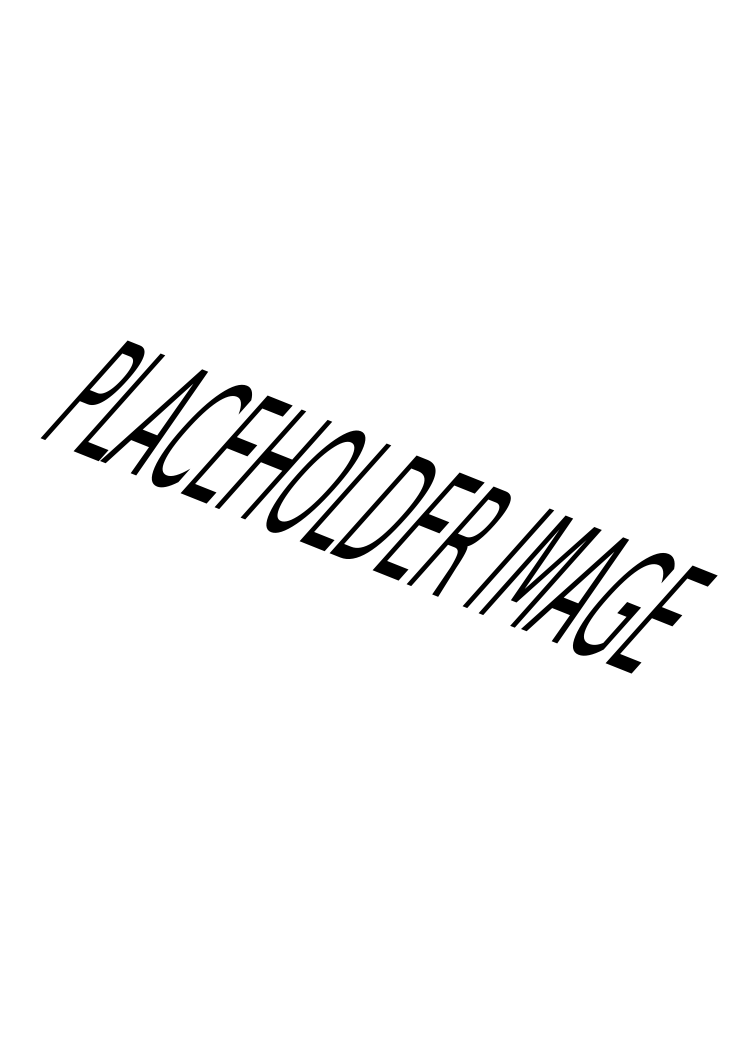
\includegraphics[width=3.0in]{./pictures/captainplaceholder.png}}
%	\caption{Pseudo code for Tabu Search Algorithm}
%	\label{fig:TSAlgorithmPseudoCode}
%\end{figure}
%\begin{figure}[htbp!]
%	\centering
%	\setlength \fboxsep{0pt}
%	\setlength \fboxrule{0.5pt}
%	\fbox{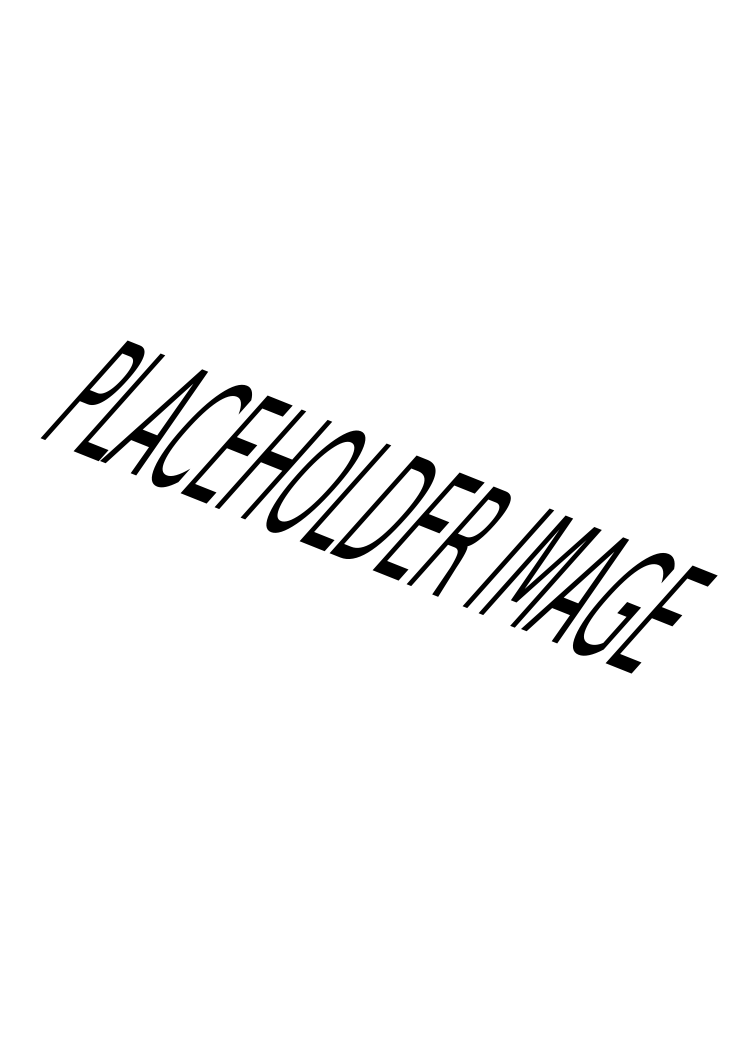
\includegraphics[width=3.8in,height=7.0in]{./pictures/captainplaceholder.png}}
%	\caption{Placeholder for algorithm data flow diagram code}
%%	\label{fig:TSFlowDiagram}
%\end{figure}
\section{Simulated Annealing}
\subsection{Overview}
Simulated Annealing (SA) is a heuristic search technique proposed in the 80's by Kirkpatrick to solve combinatorial optimisation problems. The technique is based on a natural process which is known in metallurgical as Annealing \cite{CurveFittingSA,SASingleMultiObj,TempCyclingSA,ChaosSA}. Kirkpatrick was the first to use the simulated annealing to solve optimisations problems but the basic algorithm structure was defined in by Metropolis et. al. in 1953 \cite{CurveFittingSA,VeryFastSAImageEnchancement}

Annealing is the natural process of crystallization when a solid is heated to a high temperature and then systematically cooled to a low temperature to reach a crystallized form \cite{CurveFittingSA,NewSAs,MobileRobotSA,ConstantTempSA}. This crystallized form of the solid is known the be the global minimum of the solids internal energy state. When the solid is rapidly cooled from a high temperature, the molecules have no time to reach a thermodynamic equilibrium stage \cite{CurveFittingSA,NewSAs,MobileRobotSA,ConstantTempSA}. Therefore, the molecules of the solid have high energy and the resultant structure has no real crystalline form, thus the solid energy is at a local minima \cite{CurveFittingSA,NewSAs,MobileRobotSA}. When the solid is slowly cooled in a controlled manner, the molecules are able to reach a thermal equilibrium at each temperature \cite{ChaosSA,CurveFittingSA,NewSAs,MobileRobotSA,ConstantTempSA}.

In the algorithm the energy state is the \emph{cost function} that needs to be minimised, and the molecules are the \emph{variables} which represent the solutions, and thus their state needs to be optimised to reach the desired energy state.

The following equation is the standard probability function that is used to determine when an uphill move performed by the algorithm. This function is known in the literature as the \emph{Metropolis Criterion}. 
\begin{equation}
	M_{AC} =
	\begin{cases}
	1, &\text{if $f(y) \leq f(x)$}\\
	exp(-\frac{\Delta E}{T_k}), &\text{otherwise}\\
	\end{cases}
\end{equation}
The function $f$ is the objective function or a function that determines the state of a given position in solution space\cite{EcoEquilSA}. The parameter $T_k$ is the temperature of the algorithm at iteration $k$ \cite{EcoEquilSA}. Finally, $\Delta E$ is the change in ``energy'' between two solutions $x$ and $y$ \cite{EcoEquilSA}.


The main purpose of the SA algorithm (like most optimization algorithms) is to minimize or maximise the cost function \cite{SASingleMultiObj}. This cost function typically evaluates a solutions desirability compared to other solutions in the immediate \emph{neighbourhood} of the algorithms current position \cite{TheoPraticalSA}. Typically a neighboring solution is only selected as the new best state if its desirability ranks hire than the current solution. When the algorithm moves to a better solution from the previous solution, the move is typically referred in the literature as a \emph{downhill} move \cite{CurveFittingSA}.

The best state isn't always selected, in some case the algorithm is also able to move to solutions which are worse than the current solution. A worse solution is only selected based on some probability which is controlled by the \emph{annealing temperature} of the algorithm \cite{TheoPraticalSA}. At a high annealing temperature the probability that the algorithm will select a bad solution is very good. As the annealing temperature decreases so does the probability that a bad solution will be selected \cite{CurveFittingSA}. When the algorithm moves to a worse solution, the move is typically in the literature referred to as a \emph{uphill} move \cite{CurveFittingSA}. Uphill moves allows the algorithm to breakout of local minima and can lead the algorithm down a different path which may ultimately result in obtaining the global optimum \cite{SASingleMultiObj}. 

The SA algorithm is also very popular due to the basic structure of the algorithm being generic\cite{VariousCoolingSA}. Therefore, applying the algorithm to other problems is relatively trivial since only small changes are required. These changes usually need to applied to the \emph{Neighborhood selection} scheme and the \emph{Cooling Schedule}\cite{VariousCoolingSA,DormRoomSA}. Both of these concepts will be discussed in the next sub section.

In this subsection we gave a brief overview of the Simulated Annealing (SA) algorithm. We briefly discussed what the algorithm is based on and how the algorithm goes about searching the solution space. We also introduced some concepts like move probability selection and annealing temperature, which forms part of the core the algorithm. In the next section we will explain some of the concepts we've touched upon in this section as well as more advanced concepts that makes the algorithm unique.

\subsection{Important Simulated Annealing characteristics}
In this section we will provide five brief discussions on the characteristics of the Simulated Annealing Algorithm that we think make the algorithm unique. We will start of with a discussion on Markov Chains. An discussion on one of the most important defining characteristic, namely the cooling schedule, will follow after the Markov Chain section. Furthermore we will discuss the importance of the initial temperature generation and what impact it has on the overall algorithm. Finally, we will end of this section with an overview on the efficiency of the algorithm.
\subsubsection{Markov Chain}
The SA Algorithm is typically modelled by using Markov chains due to each Markov chain represents a set of trails that the algorithm has executed at the same temperature.  It has been proven with the use of Markov Chain theory that SA will find the global minimum in the solution space \cite{ClusterSA}. This proof is only valid when the following properties for the underlying Markov chain hold \cite{VeryFastSAImageEnchancement}:
\begin{itemize}
\item It must be irreducible
\item It mustn't be periodic
\item The detailed balance condition must hold
\end{itemize}
Due to the above proof the SA algorithm has been applied to a wide range of optimisation problems because as long as the algorithm designer can uphold these properties the find the global optimum. Even though the algorithm will find the global optimum, the algorithm is known to take a very long time to do so.
\subsubsection{Cooling Schedule}
The Cooling Schedule / Annealing Schedule is the most defining characteristic of the SA algorithm. It is the procedure where the natural annealing process is mimicked. The temperature of the SA algorithm is a control parameter that defines how much the algorithm moves around in the solution space.

In general, when the SA algorithm temperature has a very high value most solutions that are produced from the neighborhood are accepted \cite{ClusterSA}. Thus the algorithm moves freely in the solution space with little constraints. As the temperature decreases the probability that the algorithm will select bad or just any solution gets lower. When the temperature is very low, the SA algorithm is similar to a greedy algorithm in a sense that it only accepts downhill movements\cite{ClusterSA}.

In the literature there are three annealing schedules in common use are namely \emph{the logarithmic schedule}, the \emph{geometric schedule} and the \emph{Cauchy schedule}\cite{VeryFastSAImageEnchancement,SASingleMultiObj}. 

The standard and most common used schedule is commonly known as the logarithmic schedule and is based on Boltzmann annealing \cite{VeryFastSAImageEnchancement}. The main disadvantage of this schedule is that is slow due to its logarithmic nature \cite{VeryFastSAImageEnchancement}. It also requires that moves be generated from a Gaussian distribution for it to be able to reach the global minimum\cite{SASingleMultiObj}. The logarithmic annealing function has the following form:
\begin{equation}
	T_k = \frac{T_0}{ln(k)},\text{where k is the iteration value}\\
\end{equation}

The Cauchy schedule is faster than the logarithmic schedule. Similar to the logarithmic, this schedule also has a movement requirement. Moves must be generated from a Cauchy distribution for the algorithm to be able to reach the global minimum \cite{SASingleMultiObj,VeryFastSAImageEnchancement}. The Cauchy schedule is also typically referred to as Fast annealing\cite{VeryFastSAImageEnchancement}. The schedule has the following form:
\begin{equation}
	T_k = \frac{T_0}{k}
\end{equation}

Finally, the fastest annealing schedule is known as the geometric or exponential annealing schedule \cite{SASingleMultiObj}. This schedule introduces the concept of \emph{re-annealing}. Re-annealing is a procedure by which all SA temperatures are rescaled \cite{VeryFastSAImageEnchancement}. This schedule has no move generation requirement to reach the global minimum, since there is no regious proof in the literature to prove it \cite{SASingleMultiObj}. The geometric schedule has the following form:
\begin{equation}
	T(i)=T_0exp(-C_i),\text{where C is a constant}
\end{equation}
\subsubsection{Initial temperature}
The initial temperature is a very important parameter to define in the SA algorithm, since it defines a point from which the cooling schedule will start of from. Therefore, depending on what the initial value of the temperature is the final result that the algorithm will produce can be influenced\cite{SALongestCommon,VariousCoolingSA,AutoConfigSA}.

When the initial temperature is set to a very high value the algorithm takes a long time reach a result. On the other hand if the initial temperature is set to a very low temperature the algorithm might converge to quickly and thus produce a result which may be the local minima\cite{SALongestCommon,VariousCoolingSA,AutoConfigSA}.

The initial temperature together with the cooling factor allows the algorithm designer to defines the time window for the algorithm to escape local minima, as well as the rate of convergence to an optimum solution\cite{SALongestCommon,VariousCoolingSA}.

A low initial temperature together with a small cooling factor makes the time window for the algorithm to leave a local optimum very small\cite{SALongestCommon}. With a high initial temperature and cooling factor value that is almost 1, the time window for the algorithm to leave the local optimum is much larger \cite{SALongestCommon}. 

When the algorithm is near a global optimum, a low initial temperature and low cooling factor will allow the algorithm to reach the optimum faster in the solution space. In contrast, if a high temperature and a very low cooling factor is used the algorithm will take longer to reach the optimum even tough it is near the global optimum\cite{SALongestCommon}.

\subsubsection{Move generation}
Most of the research done on the SA algorithm focuses on the annealing schedule and not so much on the move/solution/neighbourhood generation. Typically an initial solution is generated and then small changes are made to the solution to represent a new solution. The solution is said the be perturbed to the next solution. 

In research done by Tseung and Lin \cite{CurveFittingSA} a initial solution isn't modified but a move generation technique known as \emph{Pattern} search is used. Pattern search has two forms of movement namely the exploratory move and the patter move. The exploratory move continually changes the certain variables of a solution \cite{CurveFittingSA}. This is done so that it can rapidly find and identify a ``downhill'' move. The Pattern move uses the information gathered by the exploratory move to move towards the minimum of the function \cite{CurveFittingSA}.
\subsubsection{Algorithm efficiency}
The algorithm is also efficient with regards to CPU cycles when compared to the Genetic Algorithm because it only has to evaluate a certain number of moves each iteration, instead of a evaluating a whole population each iteration. Unlike Tabu Search the basic SA algorithm does not keep any memory and is therefore memory efficient, but in contrast suffers the risk that solution will cycling. Which is hwy the number of iterations spent at a temperature, since the longer the algorithm spends at a temperature the higher the probability is that solutions will cycle.
\subsection{Algorithm and Data flow}
In this section we will give the start of by providing the pseudo code of the Genetic Algorithm. We will also provide a flow diagram depicting the general search procedure flow of the algorithm. 
%\begin{figure}[h]
%	\centering
%	\setlength \fboxsep{0pt}
%	\setlength \fboxrule{0.5pt}
%	\fbox{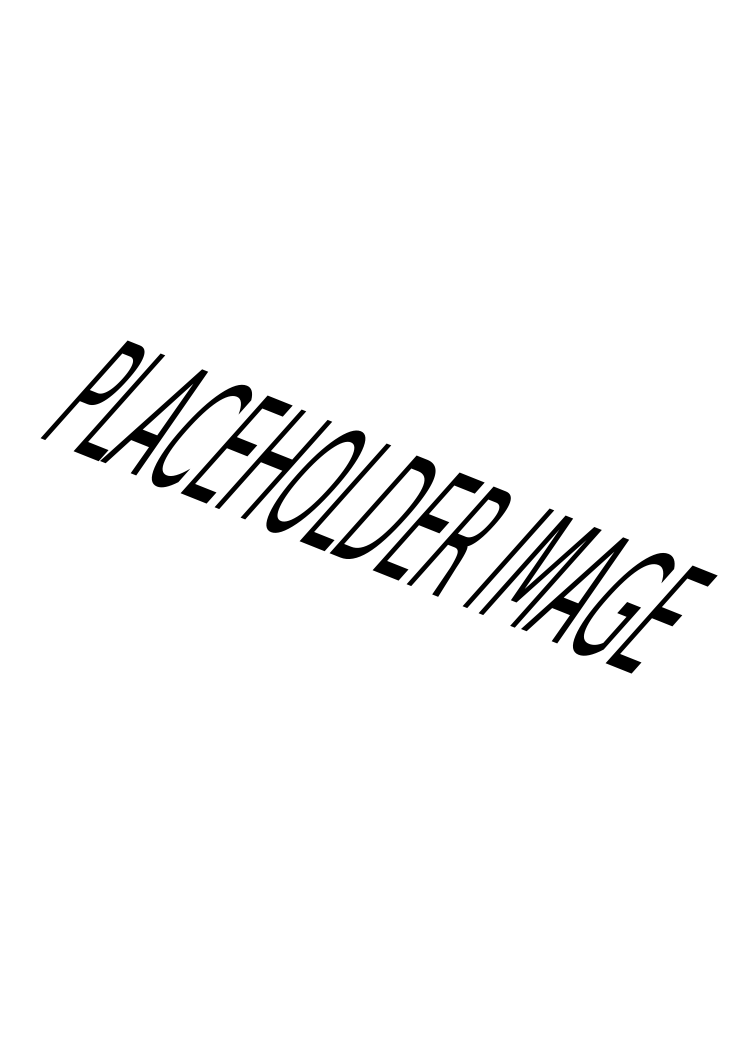
\includegraphics[width=3.0in,height=3.5in]{./pictures/captainplaceholder.png}}
%	\caption{Pseudo code for Tabu Search Algorithm}
%	\label{fig:SAAlgorithmPseudoCode}
%\end{figure}
%\begin{figure}[htbp!]
%	\centering
%	\setlength \fboxsep{0pt}
%	\setlength \fboxrule{0.5pt}
%	\fbox{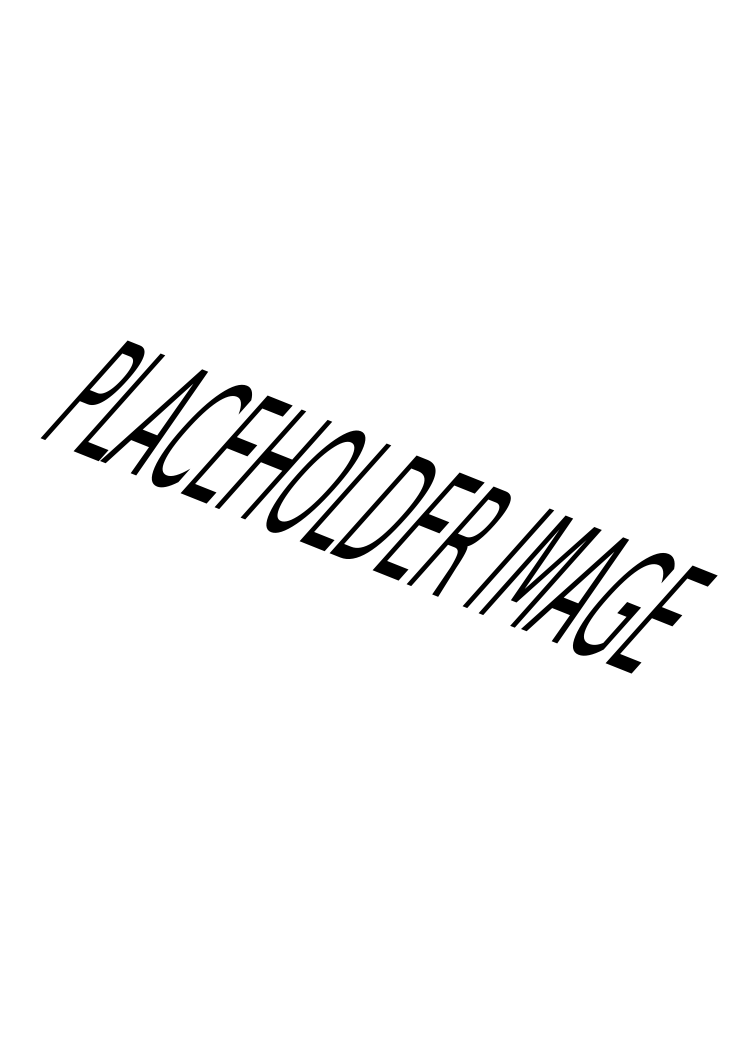
\includegraphics[width=3.8in,height=7.0in]{./pictures/captainplaceholder.png}}
%	\caption{Placeholder for algorithm data flow diagram code}
%%	\label{fig:SAFlowDiagram}
%\end{figure}
\section{Genetic Algorithm}
\subsection{Overview}
Genetic Algorithm (GA) is a stochastic search method which is based on the natural process of genetic evolution and the Darwinian concept of ``survival of the fittest'' \cite{DistributedHierarchicalGA,AcceleratingGA,AdaptiveSAGA,FamilyGA}. GA was initially developed for adaptive systems by Holland but has then, been widely used in the optimization field of study due to its effective exploration of the solution space as well as its relative success in multi-dimensional problems\cite{ParallelGASA,DistributedHierarchicalGA,FamilyGA}. The wide use of the GA algorithm can also be attributed to its generic algorithm structure as well as the ease of implementation of the algorithm \cite{FamilyGA,AdaptiveSAGA}. GA are application dependant and thus the designer needs to tailor the algorithm to his needs to obtain good results \cite{AcceleratingGA}.


The GA search procedure involves searching the solution space through artificial evolution and natural selection\cite{FamilyGA,MultiPopGA,HybridIntelliGA}. An individual or point in the solution space is known as \emph{chromosome} in the literature \cite{HumanPassiveGA}. An initial set of chromosomes (referred to in the research as the \emph{population}), are randomly generated\cite{FamilyGA,HybridIntelliGA,AcceleratingGA,MultiPopGA}. Unlike other algorithms, GA does not concentrate on one point when searching the solution space, but concentrates on a wide range of points represented by the population \cite{DistributedHierarchicalGA,FamilyGA,HybridIntelliGA}\label{GASearchPoints}. Each chromosome in the solution space represents a string encoding of the problem parameters\cite{FamilyGA}. Encoding problem parameters also attributes to the wide use of the GA since difficult mathematical problems can now be easily modelled \cite{AcceleratingGA}.

The population is artificially evolved each iteration by using a set of stochastic operators\cite{SelfAdaptiveGA}. This set consists of a selection operator, crossover operator and mutation operator\cite{SelfAdaptiveGA,MultiPopGA}. Each operator plays an important role in emulating the evolutionary process. The selection operator is in charge of applying the \emph{objective function} to each chromosome in the population \cite{AdaptiveSAGA,HumanPassiveGA}. Depending on if the selection operator is setup for maximization of minimization, each individual is ranked based on its ``fitness'' or objective function value. In accordance with the Darwinian theory, only the fittest individuals are selected from the population \cite{HumanPassiveGA}. The fittest individuals are copied and sent to the the next phase of the algorithm which is known as the \emph{Reproduction} phase \cite{HumanPassiveGA}.

Depending on how complicated the objective function is and how large the population is, the selection phase may be the most computationally expensive as well as time consuming \cite{AcceleratingGA}. The Reproduction phase mostly consists of string manipulations on the chromosome, to drive to search forward and it thus a phase which is completed quickly, especially if the string encoding is of a binary nature \cite{AcceleratingGA,AdaptiveSAGA}. These string manipulations occur through the application of the crossover and mutation operators \cite{ConstrainedGA}. The reproduction phase is where a new population is generated for the next generation to be evaluated by the selection operator. The reproduction is said to generate ``offspring'' from the selected fittest population who are in turn known as the ``parents'' of the offspring \cite{HumanPassiveGA,ConstrainedGA}. Reproduction will occur until a certain number of predefined generations is reach or a suitable solution is found to be greater/less than a certain fitness threshold that would indicate a good chromosome \cite{GATSP}.

There are two basic forms of the GA where both forms differ in the way that offspring and parents are handled \cite{FamilyGA}. The one form is called the \emph{generational} GA  and the other form is known as the \emph{steady-state} GA \cite{GeostatisticalGA,FamilyGA}. With the generational GA the offspring aren't immediately used in the next generation, instead they are kept in a pool until the pool reaches a certain size \cite{FamilyGA}. The offspring are then used to replace the parents entirely in the next generation \cite{FamilyGA}. In the steady-state GA the offspring are continually integrated with the population, thus offspring and parents occupy the same population pool every generation \cite{GeostatisticalGA,FamilyGA}.

The GA search process moves around in the search space using probabilistic rules rather than deterministic rules \cite{FamilyGA}. The probabilistic transition rules aid the algorithm to avoid local optima regions in the solution space \cite{HybridIntelliGA}. 

Some sequential search algorithms require that the objective function be differentiable \cite{ConstrainedGA}. These sequential algorithms use the derivative to obtain gradient information so that they can move in the solution space \cite{ConstrainedGA,SelfAdaptiveGA}. The derivative of the objective function may be used in to increase the efficiency of the GA but is by no means a core requirement of the algorithm \cite{ConstrainedGA,HybridIntelliGA,SelfAdaptiveGA}. GA makes no assumptions about the solution space and primarily works on the information provided by the objective function \cite{ConstrainedGA,HybridIntelliGA}. 

In this section we gave a overview of the Genetic Algorithm. We introduced the core concepts on which the algorithm is based upon as well as defined how the algorithm searches for solutions in a given domain. In the next section we will provide the pseudo code for the basic algorithmic structure as well as a flow diagram of the search procedure.

\subsection{Important Genetic Algorithm characteristics}
In this section we will give an overview on characteristics which make the GA search procedure unique. We will start of by discussing initial population generation, after which we will discuss the core operators that the GA uses. We will end of this section with a discussion on the efficiency of the GA.
\subsubsection{Initial Population Generation}
Initial population generation is the very first activity that the GA performs. Out of this population potential mating candidates are selected based on their fitness which indicates the desirability. Generally the initial population is generated by means of randomization \cite{SelfAdaptiveGA}. Since the algorithm searches multiple points simultaneously in the solution space, it is desirable that the initial population have a wide diversity with regard to the solution they represent \cite{CombinedBranchBoundGA,DistributedHierarchicalGA}. By controlling the initial population generation we can control, to a small degree, the amount of exploration the algorithm does initially as well as avoid premature convergence \cite{CombinedBranchBoundGA}. Therefore, care must be taken in the selection of the particular randomization scheme that will be used to generate solutions.

In a survey done by Andrea Reese, two randomization schemes are defined namely pseudo-random number generators (PRNGs) and quasi-random number generators (QRNGs). PRNGs where found to be heavily problem dependant, improving the search efficiency in some instances and in other instances having no considerable impact. QRNGs on the other hand, were shown to significantly improve the final solution produced by the GA as well as lowering the number of generations for the solution to be obtained \cite{RandomNumberGA}.

Not all GA algorithm use randomization entirely for their initial population generation. In research done by Amit Nagar, Sunderesh S. Heragu and Jorge Haddock an algorithm is presented that generates an initial population through some aid of a branch-and-bound algorithm. The branch-and-bound algorithm provides the GA with an upper bound of acceptable solution in the solution space. The initial population is then randomly generated in the constrained space defined by the upper bound\cite{CombinedBranchBoundGA}.
\subsubsection{Selection Operator}
The Selection operator is the first operator to be applied to the population after each generation. This operator is in charge of evaluating the current population to determine which individuals will survive and which will be ``killed'' off \cite{CoactiveFuzzyGA,CombinedBranchBoundGA,ConstrainedGA}. The individuals who survive and thus have the highest fitness are moved to a ``mating pool'' \cite{HumanPassiveGA}. Individuals from this mating pool will be used in the the reproduction phase to generate a new population \cite{AdaptiveSAGA,AcceleratingGA}.

By favouring high fitness individuals above low fitness individuals the operator guides the search towards better high quality solutions \cite{ConstrainedGA}. But care must be taken if the operator is to keen on high quality individuals since it may eliminate diversity in the population and thus result in premature convergence for certain problems \cite{ConstrainedGA}. If the solution space is known to have only one optimum, then a strict selection policy may be used, therefore directing the search into a gradient based direction \cite{ConstrainedGA}. In contrast, with a solution space that is known to have multiple optima, a forgiving selection policy might be more favourable since it allows the solution space to be more widely explored \cite{ConstrainedGA}.

The most widely adopted selection scheme is known as the \emph{Roulette Wheel} selection scheme \cite{ConstrainedGA,GeostatisticalGA,HybridBaldwinGA,CoactiveFuzzyGA}. With this scheme an individual is selected based on a probability defined by the fitness of the individual divided by the collective fitness of the population \cite{GeostatisticalGA}.
\subsubsection{Crossover Operator}
\label{sec:crossover}
The Crossover operator is usually the first operator applied to the population in the reproduction phase. The crossover operates exclusively only on the chromosomes that are in the mating pool. This operator is the main process by which by the GA algorithm is able to diversify as well as exploit certain optimal regions \cite{CombinedBranchBoundGA,CoactiveFuzzyGA}. Crossover works by interchanging and matching two parent chromosomes randomly selected from the mating pool to produce a single chromosome known as the offspring \cite{FamilyGA,HumanPassiveGA,CoactiveFuzzyGA}. Since two chromosomes are combined or partially changed, some historical information is retained in the new chromosome \cite{FamilyGA}.

In some algorithms like for instance the one presented in Nagar et. al., before the crossover operator is applied to the two parent chromosomes, the parents are first evaluated to determine if they represent suboptimal regions. If the either of the parents are from a suboptimal region, a disruption operator is applied that interchanges certain domain specific information between the parents. After the disruption operator is applied the crossover operator is applied \cite{CombinedBranchBoundGA}.

There are a variety of ways with which values are interchanged between chromosomes in the crossover operation i.e, Fixed point crossover, Two Point Crossover, Uniform Crossover and Gaussian Crossover. Fixed point crossover operates on binary parents where by a point is selected in one parent and then all other bits are replaced by the other parents bits \cite{HumanPassiveGA}. Two point crossover generates two random indices's which dictates a certain segment in the one parent to be interchanged with the other parent \cite{ConstrainedGA}. Uniform crossover is the most basic of all crossovers since it randomly selects bits from one parent to be replaced by another parents bits and is usually used when a large solution space must be search\cite{ParallelGASA,GeostatisticalGA}. Finally, the Gaussian crossover, interchanges bits between parents based on a Gaussian distribution \cite{ParallelGASA,GeostatisticalGA}. Depending on the state of the algorithm, crossover operators can also be interchanged or even paired if the algorithm needs better search performance for large or small solution spaces \cite{HetergeneousGA,ParallelGASA}.

Note, in all above crossovers it is assumed that the chromosomes are bit encoded, but these crossover do require them to be. All these crossover operators are able to work on any encoding, it just depends on what is considered to be a ``bit'' if a non-binary encoding is used. 

\subsubsection{Mutation Operator}
The mutation operator is a probabilistic operator, which means it is applied infrequently and thus only with a certain probability will it be applied to parent solution. The operator typically changes some small in the solution regardless of the fitness of the chromosome \cite{HybridBaldwinGA,HumanPassiveGA}.

Given enough time, the mutation operator enables the algorithm to search the entire search space \cite{FamilyGA}. The operator also aids the algorithm with regard to escaping local optima in the solution space \cite{FamilyGA}.

Due to the way the crossover works, some information may be lost when it is replaced by another chromosomes bits \cite{AcceleratingGA,ConstrainedGA}. Mutation is a source of new information which is continuously inserted into the algorithm, hence it works against information loss \cite{CoactiveFuzzyGA,AcceleratingGA,ConstrainedGA}. Usually, the mutation operator has no previous information on the chromosome it is mutating, thus it is entirely possible that the mutation may modify the chromosome for the worse \cite{AcceleratingGA}. A worse solution might lead the algorithm out of local optima or lead it down a new path to find the global optima, but this isn't always the case and thus in the literature the probability of the mutation operator is set to be very low \cite{AdaptiveSAGA,FamilyGA,ConstrainedGA}.

In a survey done by Engelbrecht another mutation operator is dicussed. Instead of mutating a small part of a randomly selected chromosomes, this operator generates new offspring to be inserted back into the population. The operator randomly generates a new chromosome and then using any of the previous discussed crossover operators (see page~\pageref{sec:crossover}) a 

The mutation operator isn't always simple random operations. In research done by Il-kwon Jeong and Ju-jang Lee, a mutation operator is presented that incorporates the Simulated Annealing algorithm. Th SA mutation operator generates a new chromosome whose fitness is also calculated. If the new chromosome fitness is worse than the chromosome to be mutated, then depending on the SA mutation temperature as well cooling schedule , the newly generated chromosome might replace the chromosome to be mutated. Otherwise, if the new chromosome has a better fitness than the chromosome to be mutated, then it is replaced \cite{AdaptiveSAGA}.

\subsubsection{Elitism Operator}
The elitist operator differs from the crossover and mutation operator in a sense that, it doesn't modify the chromosomes in any way. Instead, the operator works on the population \cite{PatternDetectionGA}. The elitist operator ensures that the best chromosomes do not get lost from one population to the next, when the crossover and mutation operators are applied \cite{HetergeneousGA}. Thus the elitist operator is only applied after the crossover and mutation operators have generated a new population. 

The elitist selects a certain number of high quality chromosomes from the parent population and transfers them in the new population without any modification from the other two operators \cite{PatternDetectionGA}. The operator does not just move parents into the new population. The operator typically replaces sub par chromosomes in the new population with the higher quality parents \cite{RealParameterGASA}. Therefore, the elitist operator helps the algorithm retain knowledge gained from previous generations and prevents the best solution from extinction \cite{DynamicPenaltyGA}. Finally, the retainment of knowledge and best solution aids the algorithm with regard to global convergence \cite{SelfAdaptiveDataMiningGA}.

\subsubsection{Algorithm Efficiency}
The GA is a powerful, yet simple algorithm and tends to find good solutions given enough time. But the algorithm does has its disadvantages. One of the major disadvantages occurs when the GA is applied to problems which have very large solution spaces. In these problem, the population size is a very sensitive parameter. If the population is too small the algorithm won't have enough diversity to search and tends to premature converge. 

A large population is preferred in large problem spaces, but then the algorithm is very computationally expensive since more time is spent evaluating than evolving new populations and the speed of the algorithm convergence decreases drastically. Hence, the population size must be fine tuned to achieve optimal performance in large problem spaces

Another disadvantage of GA, is that it is memory intensive, most sequential algorithms search on a single point bases through the solution space. As discussed above(see page ~\pageref{GASearchPoints}), searches multiple points simultaneously and therefore requires more memory the keep track of all the possible solutions.

Finally, the algorithm has some sort of hill-climbing through the mutation operator, but the probability of the mutation operator is far too low for the algorithm to be considered to have a real hill-climbing capability.
\subsection{Algorithm and Data flow}
In this section we will give the start of by providing the pseudo code of the Genetic Algorithm. We will also provide a flow diagram depicting the general search procedure flow of the algorithm. 
%Fuzzy genetic optimization on performance-based seismic design of reinforced concrete bridge piers with single-column type page  10 for flow chart
%\begin{figure}[h]
%	\centering
%	\setlength \fboxsep{0pt}
%	\setlength \fboxrule{0.5pt}
%	\fbox{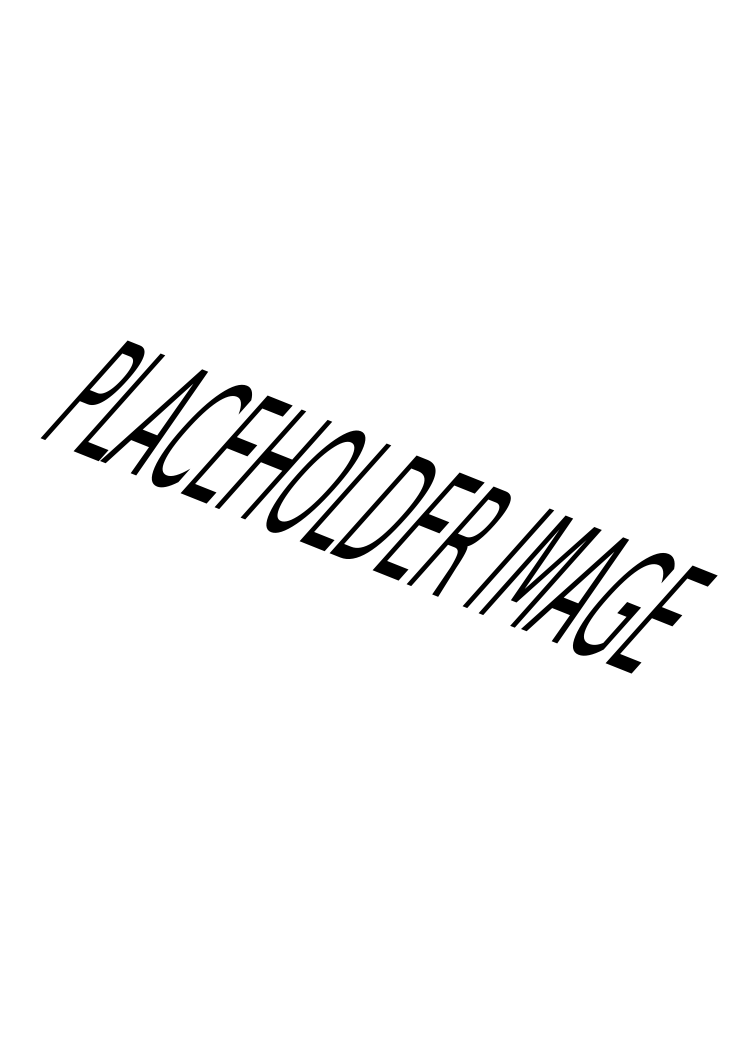
\includegraphics[width=3.0in,height=3.7in]{./pictures/captainplaceholder.png}}
%	\caption{Pseudo code for Tabu Search Algorithm}
%	\label{fig:GAlgorithmPseudoCode}
%\end{figure}
%\begin{figure}[htbp!]
%	\centering
%	\setlength \fboxsep{0pt}
%	\setlength \fboxrule{0.5pt}
%	\fbox{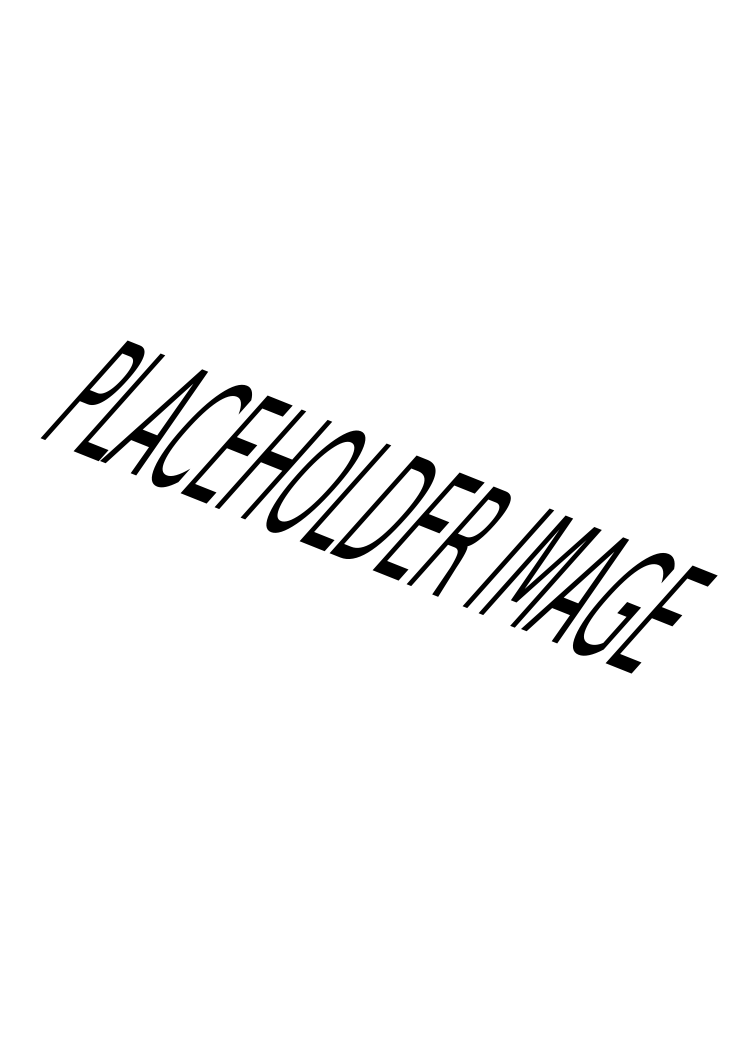
\includegraphics[width=3.8in,height=7.0in]{./pictures/captainplaceholder.png}}
%	\caption{Placeholder for algorithm data flow diagram code}
%%	\label{fig:GAFlowDiagram}
%\end{figure}
\section {Summary}
